\documentclass[a4paper]{article}
\usepackage[T1]{fontenc}			% pacchetto per \chapter
\usepackage[italian]{babel}
\usepackage[italian]{isodate}  		% formato delle date in italiano
\usepackage{graphicx}				% gestione delle immagini
\usepackage{amsfonts}
\usepackage{booktabs}				% tabelle di qualità superiore
\usepackage{mathrsfs, amsmath}				% pacchetto matematica
\usepackage{mathtools}				% per sottolineare sotto le equazioni
\usepackage{stmaryrd} 				% per '\llbracket' e '\rrbracket'
\usepackage{amsthm}					% teoremi migliorati
\usepackage{enumitem}				% gestione delle liste
\usepackage{pifont}					% pacchetto con elenchi carini
\usepackage{enumitem}				% pacchetto per elenchi con lettere dell'alfabeto
\usepackage{cancel}					% per cancellare delle espressioni matematiche
\usepackage{listings}				% implementa codice di programmazione
\usepackage{mathalpha}
\usepackage{caption}


\usepackage[x11names]{xcolor}		% pacchetto colori RGB
% Link ipertestuali per l'indice
\usepackage{xcolor}
\usepackage[linkcolor=black, citecolor=blue, urlcolor=cyan]{hyperref}
\hypersetup{
	colorlinks=true
}

% Colour code style
\definecolor{codegreen}{rgb}{0,0.6,0}
\definecolor{codegray}{rgb}{0.5,0.5,0.5}
\definecolor{codepurple}{rgb}{0.58,0,0.82}
\definecolor{backcolour}{rgb}{0.95,0.95,0.92}

\lstdefinestyle{MATLAB}{
	backgroundcolor=\color{backcolour},   
	commentstyle=\color{codegreen},
	keywordstyle=\color{magenta},
	numberstyle=\tiny\color{codegray},
	stringstyle=\color{codepurple},
	basicstyle=\ttfamily\footnotesize,
	breakatwhitespace=false,         
	breaklines=true,                 
	captionpos=b,                    
	keepspaces=true,                 
	numbers=left,                    
	numbersep=5pt,                  
	showspaces=false,                
	showstringspaces=false,
	showtabs=false,                  
	tabsize=2
}
\lstset{style=MATLAB}

%\usepackage{showframe}				% visualizzazione bordi
%\usepackage{showkeys}				% visualizzazione etichetta

\newtheorem{theorem}{\textcolor{Red3}{\underline{Teorema}}}
\newtheorem{lemma}{Lemma}
\renewcommand{\qedsymbol}{QED}
\newcommand{\exec}[1]{\llbracket #1\:\rrbracket}
\newcommand{\dquotes}[1]{``#1''}
\newcommand{\longline}{\noindent\rule{\textwidth}{0.4pt}}

\begin{document}
	\author{Università degli Studi di Verona}
	\title{Soluzione - Simulazione di Elaborazione di segnali e immagini}
	\date{{\Large 26 Marzo 2021}}
	\maketitle
	
	\section{Soluzione Esercizio}
	
	Il segnale graficamente è composto da due box all'estremo e al centro da una box sommata ad un triangolo. Quindi nel dominio delle frequenze:
	\begin{equation*}
		X\left(\mu\right) = \underbrace{4\Pi\left(\dfrac{\mu + 5}{2}\right) + 4\Pi\left(\dfrac{\mu - 5}{2}\right)}_{\text{Box esterne}} + \overbrace{2\Pi\left(\dfrac{\mu}{6}\right) + 2\Lambda\left(\dfrac{\mu}{2}\right)}^{\text{Box e triangolo centrale}}
	\end{equation*}
	Nel dominio del tempo:
	\begin{equation*}
		\begin{array}{lll}
			x\left(t\right) & = & 4 \cdot 2 \mathrm{sinc}\left(2t\right) e^{j 2 \pi 5 t} + 4 \cdot 2 \mathrm{sinc}\left(2t\right) e^{-j 2 \pi 5 t} + 2 \cdot 6\mathrm{sinc}\left(6t\right) + 2 \cdot 2\mathrm{sinc}^{2}\left(2t\right) \\
			\\
			& = & 8\cdot\mathrm{sinc}\left(2t\right) e^{j 2 \pi 5 t} + 8\cdot\mathrm{sinc}\left(2t\right) e^{-j 2 \pi 5 t} + 12\cdot\mathrm{sinc}\left(6t\right) + 4\cdot\mathrm{sinc}^{2}\left(2t\right) \\
			\\
			& = & 8 \cdot \mathrm{sinc}\left(2t\right) \cdot \left[e^{j 2 \pi 5 t} + e^{-j 2 \pi 5 t}\right] + 12\cdot\mathrm{sinc}\left(6t\right) + 4\cdot\mathrm{sinc}^{2}\left(2t\right)
		\end{array}
	\end{equation*}\newpage
	
	\subsection*{\textcolor{Green4}{\textbf{\emph{\underline{Filtro passa basso $\boldsymbol{a\left(t\right)}$}}}}}
	
	Il filtro passo basso ideale è una box e la frequenza di taglio rappresenta metà della larghezza. Essa rappresenta una convoluzione nel dominio del tempo e una moltiplicazione nel dominio delle frequenze. Graficamente, si eliminano le box esterne e si mantiene il box e il triangolo centrale diminuendo la larghezza:
	\begin{equation*}
		\begin{array}{lll}
			\text{Dominio nelle frequenze} 	& \longrightarrow & A\left(\mu\right) = X\left(\mu\right) \cdot \Pi\left(\dfrac{\mu}{4}\right) = 2\Pi\left(\dfrac{\mu}{4}\right) + 2\Lambda\left(\dfrac{\mu}{2}\right) \\
			\\
			\text{Dominio nel tempo} 		& \longrightarrow & a\left(t\right) = x\left(t\right) * 4\mathrm{sinc}\left(4t\right) = 8\mathrm{sinc}\left(4t\right) + 4\mathrm{sinc}^{2}\left(2t\right)
		\end{array}
	\end{equation*}
	\begin{figure}[!htp]
		\centering
		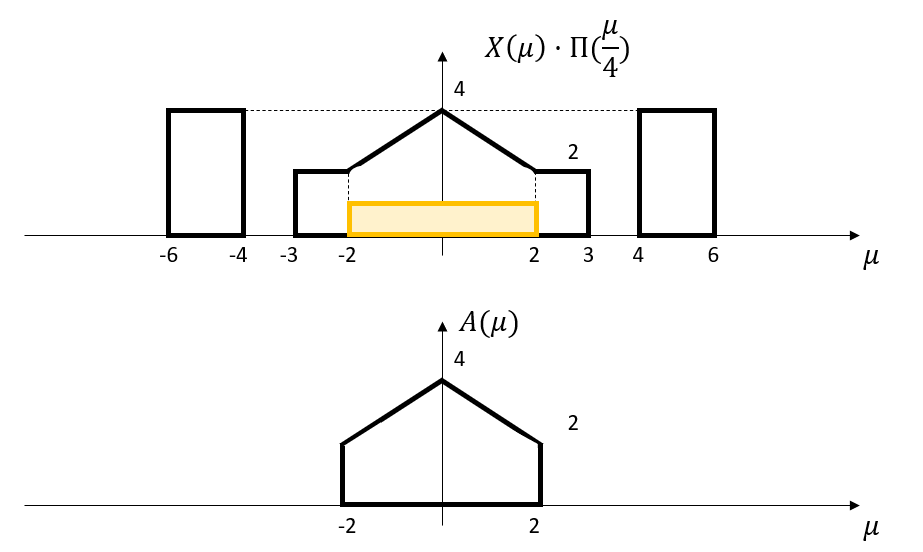
\includegraphics[width=\textwidth]{img/fig_1.png}
		\caption*{Rappresentazione grafica del segnale $A\left(\mu\right)$ nel dominio delle frequenze.}
	\end{figure}\newpage

	\subsection*{\textcolor{Green4}{\textbf{\emph{\underline{Moltiplicazione nel tempo $\boldsymbol{b\left(t\right)}$}}}}}
	
	La moltiplicazione di due segnali nel dominio del tempo corrisponde ad una convoluzione nel dominio delle frequenze. Prima di tutto si rappresenta in tale dominio il segnale in entrata:
	\begin{equation*}
		\begin{array}{lll}
			\text{Dominio nel tempo} 		& \longrightarrow & \cos\left(2 \pi 4 t\right) \\
			\\
			\text{Dominio nelle frequenze} 	& \longrightarrow &  \dfrac{1}{2}\left(\delta\left(\mu + 4\right) + \delta\left(\mu - 4\right)\right)
		\end{array}
	\end{equation*}
	Si sviluppa analiticamente la convoluzione nel dominio delle frequenze:
	\begin{equation*}
		\begin{array}{lll}
			B\left(\mu\right) & = & A\left(\mu\right) * \dfrac{1}{2}\left(\delta\left(\mu + 4\right) + \delta\left(\mu - 4\right)\right) \\
			\\
			& = & \displaystyle\int_{-\infty}^{\infty} A\left(\tau\right) \cdot \dfrac{1}{2}\left(\delta\left(\mu + 4 - \tau\right) + \delta\left(\mu - 4 - \tau\right)\right) \: \mathrm{d}\tau \\
			\\
			& = & \dfrac{1}{2} \cdot \left(\displaystyle\int_{-\infty}^{\infty} A\left(\tau\right) \cdot \delta\left(\mu + 4 - \tau\right) \: \mathrm{d}\tau + \displaystyle\int_{-\infty}^{\infty} A\left(\tau\right) \cdot \delta\left(\mu - 4 - \tau\right) \: \mathrm{d}\tau\right) \\
			\\
			& \downarrow & \text{Proprietà di setacciamento} \\
			\\
			& = & \dfrac{1}{2} A\left(\mu+4\right) + \dfrac{1}{2} A\left(\mu-4\right) \\
			\\
			& = & \dfrac{1}{2} \left[2\Pi\left(\dfrac{\mu + 4}{4}\right) + 2\Lambda\left(\dfrac{\mu + 4}{2}\right)\right] + \dfrac{1}{2} \left[2\Pi\left(\dfrac{\mu - 4}{4}\right) + 2\Lambda\left(\dfrac{\mu - 4}{2}\right)\right] \\
			\\
			& = & \Pi\left(\dfrac{\mu + 4}{4}\right) + \Lambda\left(\dfrac{\mu + 4}{2}\right) + \Pi\left(\dfrac{\mu - 4}{4}\right) + \Lambda\left(\dfrac{\mu - 4}{2}\right)
		\end{array}
	\end{equation*}
	Nel dominio del tempo:
	\begin{equation*}
		b\left(t\right) = 4\mathrm{sinc}\left(4t\right)e^{j 2 \pi 4 t} + 2\mathrm{sinc}^{2}\left(2t\right)e^{j 2 \pi 4 t} + 4\mathrm{sinc}\left(4t\right)e^{-j 2 \pi 4 t} + 2\mathrm{sinc}^{2}\left(2t\right)e^{-j 2 \pi 4 t}
	\end{equation*}
	\begin{figure}[!htp]
		\centering
		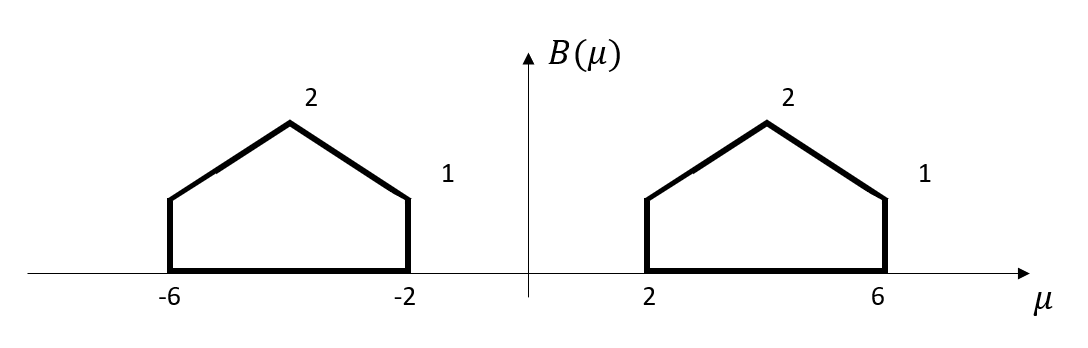
\includegraphics[width=\textwidth]{img/fig_2.png}
		\caption*{Rappresentazione grafica del segnale $B\left(\mu\right)$ nel dominio delle frequenze.}
	\end{figure}\newpage
	
	\subsection*{\textcolor{Green4}{\textbf{\emph{\underline{Campionatore $\boldsymbol{c\left(t\right)}$}}}}}
	
	Il campionatore ha una frequenza a scelta e quest'ultima deve essere fatta cercando di evitare il fenomeno di aliasing. Guardando il grafico, la prima frequenza ammessa è $12$ Hz. Quindi, dato che il campionamento nel domino del tempo corrisponde ad una moltiplicazione e ad una convoluzione nel domino delle frequenze:
	\begin{equation*}
		\begin{array}{lll}
			\text{Dominio nel tempo} 		& \longrightarrow & c\left(t\right) = b\left(t\right) \cdot \displaystyle\sum_{n} \delta\left(\dfrac{t - n}{12}\right) \\
			\\
			\text{Dominio nelle frequenze} 	& \longrightarrow & C\left(\mu\right) = B\left(\mu\right) * 12\displaystyle\sum_{n} \delta\left(\mu-12n\right)
		\end{array}
	\end{equation*}
	Si sviluppa analiticamente la convoluzione nel dominio delle frequenze:
	\begin{equation*}
		\begin{array}{lll}
			C\left(\mu\right) & = & B\left(\mu\right) * 12\displaystyle\sum_{n} \delta\left(\mu-12n\right) \\
			\\
			& = & \displaystyle\int_{-\infty}^{\infty} B\left(\tau\right) \cdot 12\displaystyle\sum_{n} \delta\left(\mu-12n-\tau\right) \: \mathrm{d}\tau \\
			\\
			& = & 12 \cdot \displaystyle\int_{-\infty}^{\infty} B\left(\tau\right) \cdot \displaystyle\sum_{n} \delta\left(\mu-12n-\tau\right) \: \mathrm{d}\tau \\
			\\
			& \downarrow & \text{Proprietà di setacciamento} \\
			\\
			& = & 12 \cdot \displaystyle\sum_{n} B\left(\mu-12n\right)
		\end{array}
	\end{equation*}
	\begin{figure}[!htp]
		\centering
		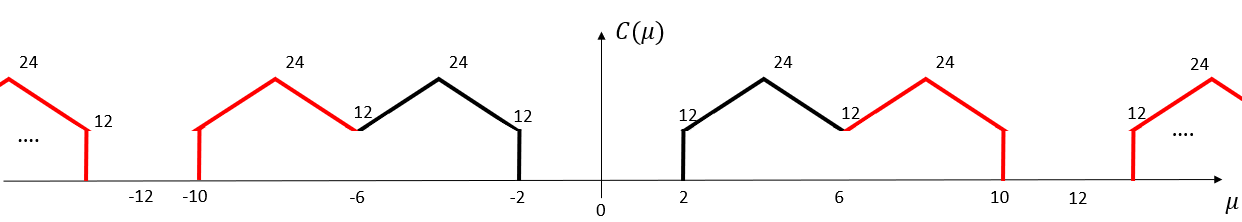
\includegraphics[width=\textwidth]{img/fig_3.png}
		\caption*{Rappresentazione grafica del segnale $C\left(\mu\right)$ nel dominio delle frequenze.}
	\end{figure}\newpage

	\subsection*{\textcolor{Green4}{\textbf{\emph{\underline{Filtro passa basso $\boldsymbol{d\left(t\right)}$}}}}}
	
	Il filtro passo basso ideale è una box e la frequenza di taglio rappresenta metà della larghezza. Essa rappresenta una convoluzione nel dominio del tempo e una moltiplicazione nel dominio delle frequenze. Graficamente, si eliminano i segnali in più creati con il campionatore. Il dominio delle frequenze quindi corrisponde al segnale $B\left(\mu\right)$:
	\begin{equation*}
			D\left(\mu\right) = C\left(\mu\right) \cdot \Pi\left(\dfrac{\mu}{12}\right) = \Pi\left(\dfrac{\mu + 4}{4}\right) + \Lambda\left(\dfrac{\mu + 4}{2}\right) + \Pi\left(\dfrac{\mu - 4}{4}\right) + \Lambda\left(\dfrac{\mu - 4}{2}\right)
	\end{equation*}
	Idem per il domino nel tempo:
	\begin{equation*}
		a\left(t\right) = c\left(t\right) * 12\mathrm{sinc}\left(12t\right) = 4\mathrm{sinc}\left(4t\right)e^{j 2 \pi 4 t} + 2\mathrm{sinc}^{2}\left(2t\right)e^{j 2 \pi 4 t} + 4\mathrm{sinc}\left(4t\right)e^{-j 2 \pi 4 t} + 2\mathrm{sinc}^{2}\left(2t\right)e^{-j 2 \pi 4 t}
	\end{equation*}
	\begin{figure}[!htp]
		\centering
		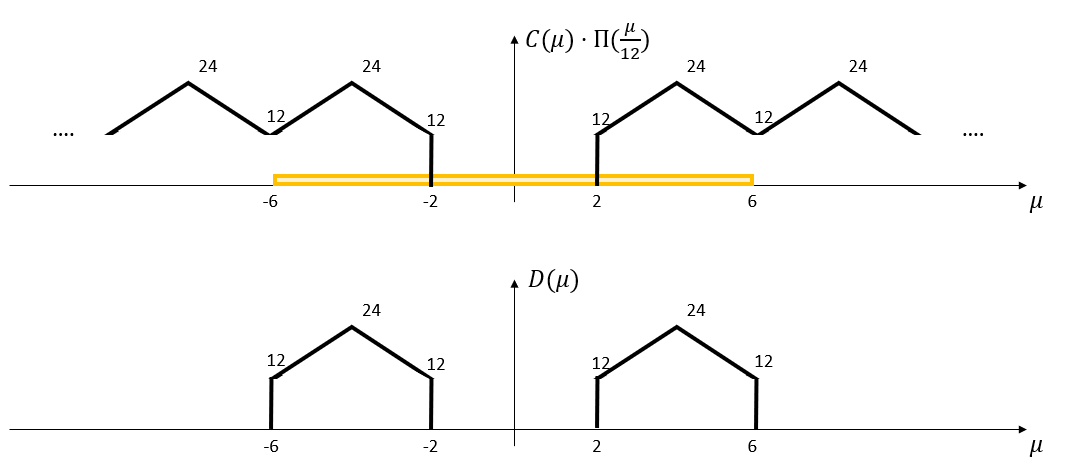
\includegraphics[width=\textwidth]{img/fig_4.png}
		\caption*{Rappresentazione grafica del segnale $D\left(\mu\right)$ nel dominio delle frequenze.}
	\end{figure}\newpage

	\section{Soluzione Esercizio}
	
	Prima di procedere alla convoluzione dei segnali, si ottiene la forma analitica dei segnali nel dominio delle frequenze:
	\begin{equation*}
		\begin{array}{lll}
			H\left(\mu\right) & = & 2\Pi\left(\dfrac{\mu - 1}{2}\right) \\
			\\
			X\left(\mu\right) & = & \delta\left(\mu - 1\right) + \delta\left(\mu - 2\right) + \Pi\left(\dfrac{\mu - 4.5}{1}\right)
		\end{array}
	\end{equation*}
	Si descrive graficamente il segnale assumendo che in $h\left(0\right)$ il risultato sia zero, quindi con $t < 1$, non vi è intersezione tra i segnali e il segnale $y$ non esiste;:
	\begin{enumerate}[label=\alph*)]
		\item $1 \le t < 2$, vi è intersezione con il primo impulso, il prodotto tra i segnali genera impulsi di ampiezza $2$. Quindi, l'integrale vale $2$: $y\left(1 \le t < 2\right) = 2$;
		
		\item $2 \le t < 3$, vi è intersezione con entrambi gli impulsi, il prodotto tra i segnali genera impulsi di ampiezza $4$. Quindi, l'integrale vale $4$: $y\left(2 \le t < 3\right) = 4$;
		
		\item $3 \le t < 4$, vi è intersezione con il secondo impulso, il prodotto tra i segnali genera impulsi di ampiezza $2$. Quindi, l'integrale vale $2$: $y\left(3 \le t < 4\right) = 2$;
		
		\item $t = 4$, vi è intersezione ma il prodotto tra i segnali è zero. L'integrale vale quindi $0$: $y\left(4\right) = 0$. Nel caso in cui si consideri gli estremi positivi, allora il prodotto non è zero, ma il valore in questo punto rimane a $2$: $y\left(4\right) = 2$;
		
		\item $t = 5$ vi è un'intersezione con il segnale, il prodotto tra i segnali produce una box di ampiezza $2$ e base $1$. L'integrale è pari all'area del rettangolo, cioè $2$: $y\left(5\right)=2$;
		
		\item $t = 6$ come per $t = 5$ vi è un'intersezione tra i segnali. Dato che è identico, di nuovo l'integrale vale $2$: $y\left(6\right)=2$;
		
		\item $t = 7$ come per il caso $t = 4$, vi è intersezione ma il prodotto tra i segnali è zero. Quindi, l'integrale vale $0$: $y\left(7\right) = 0$.
	\end{enumerate}
	Con $t>7$ non vi è intersezione di segnali e $y$ non esiste.\newpage
	\begin{figure}[!htp]
		\centering
		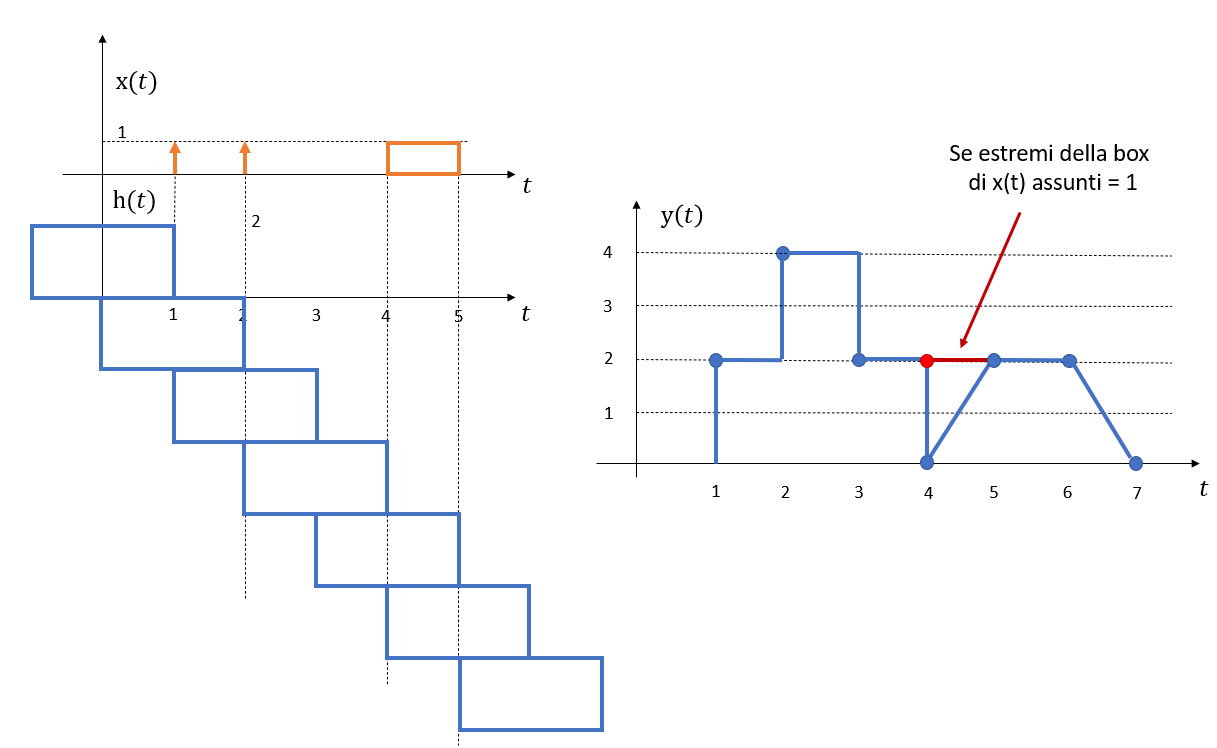
\includegraphics[width=\textwidth]{img/fig_5.png}
		\caption*{Rappresentazione grafica della convoluzione tra $x\left(t\right)$ e $h\left(t\right)$.}
	\end{figure}
	
	\noindent
	Adesso si rappresenta graficamente il caso in cui venga effettuata questa differenza:
	\begin{equation*}
		w\left(t\right) = \Pi\left(\dfrac{t-4}{6}\right) - y\left(t\right)
	\end{equation*}
	Come sempre, prima di eseguire la differenza, è consigliato capovolgere il segnale $y\left(t\right)$ e poi eseguire una banale somma così da non sbagliare i calcoli.
	\begin{figure}[!htp]
		\centering
		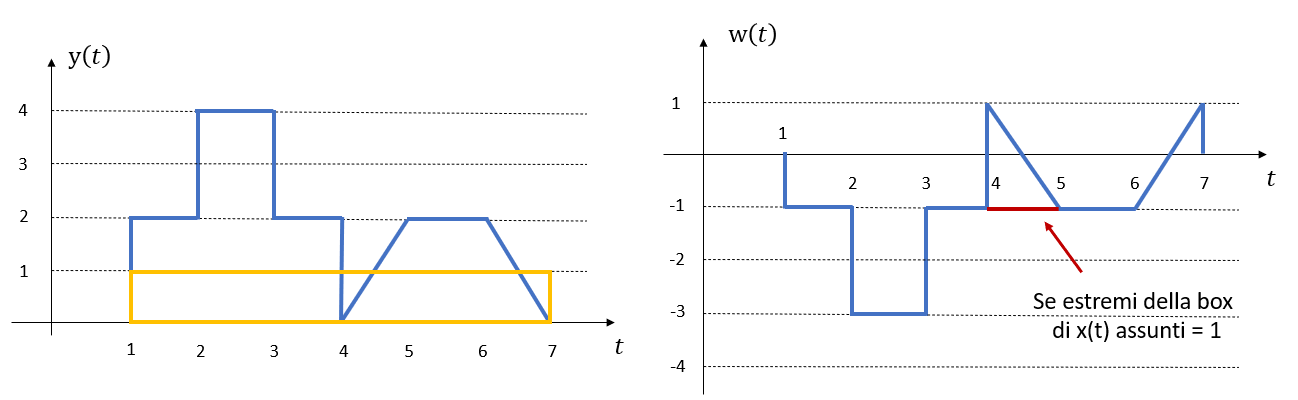
\includegraphics[width=\textwidth]{img/fig_6.png}
		\caption*{Rappresentazione grafica del segnale $w\left(t\right)$.}
	\end{figure}\newpage

	\section{Soluzione Esercizio}
	
	\subsection*{\textcolor{Green4}{\emph{\underline{Risposta prima domanda}}}}
	
	È evidente che l'immagine di sinistra sia quella con più dettagli rispetto all'immagine \emph{b}. Data questa particolarità, è stato visto che le immagini più dettagliate hanno uno spettro di ampiezza con frequenze molto più variabili. Ovvero, non vi sono frequenze basse dominanti. Si prenda come esempio le due immagini estratte dalle slide del corso:
	\begin{figure}[!htp]
		\centering
		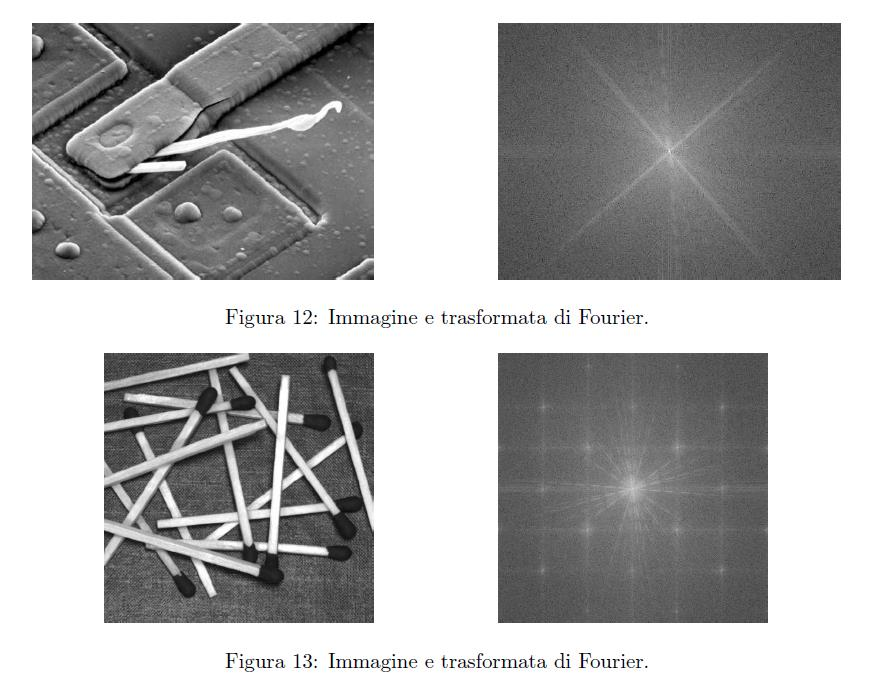
\includegraphics[width=\textwidth]{img/fig_7.png}
	\end{figure}
		
	\noindent
	È possibile notare come gli spettri di ampiezza abbiano abbiano un certo equilibrio di frequenze alte\footnote{Le frequenze alte, nello spettro di ampiezza, sono rappresentate da un nero più intenso.} e basse\footnote{Le frequenze basse, nello spettro di ampiezza, sono rappresentate da un bianco più intenso.}.\newline
	
	\noindent
	Al netto di queste considerazioni, è corretto supporre che l'immagine \emph{a} abbia uno spettro di ampiezza identico alla figura 1, piuttosto che alla figura 2.\newpage
	
	\subsection*{\textcolor{Green4}{\emph{\underline{Risposta seconda domanda}}}}
	
	Come veniva spiegato nella risposta precedente, è evidente che l'immagine di sinistra abbia una quantità di informazioni maggiore rispetto a quella di destra. Quest'ultima, infatti, ha subito un certo tipo di operazione di filtraggio. Le operazioni che possono essere state applicate sono 3:
	\begin{itemize}
		\item Filtro passa-basso ideale;
		\item Filtro di Butterworth;
		\item Filtro passa-basso Gaussiano.
	\end{itemize}
	La soluzione ottimale per ottenere tale risultato sarebbe l'applicazione di un filtro passa-basso Gaussiano così da non ottenere fenomeni di \emph{ringing}. Tuttavia, per valori di $\sigma$ non troppo alti, andrebbe bene anche un filtro di Butterworth. Infine, il filtro passa-basso ideale rimane l'ultima scelta poiché con tale filtro si manifesterebbe certamente il fenomeno di \emph{ringing}.
	
	Ovviamente, dopo aver applicato uno dei tre filtri sullo spettro di ampiezza, si esegue l'antitrasformata di Fourier così da rappresentare l'immagine.\newline
	
	\noindent
	Infine, lo spettro di fase \underline{non} necessita di modifiche poiché esso entra in gioco solamente nel momento in cui ci sono traslazioni o rotazioni.
\end{document}